%!TEX root = ../../master.tex

\section{Microservice Architecture}
Microservices have been one of the most hyped architectural styles for the past couple of years. A survey done by Nginx in November 2015 showed that: 
\textit{"nearly 70\% of organizations are either using or investigating microservices, with nearly 1/3 currently using them in production"} \cite[p. 6]{nginx2016future}. The respondent pool consisted of 1,825 NGINX community members such as developers, application architects, DevOps, CIO/CTOs, and system administrators. \\

\noindent
Microservices are not a completely new way of architecting software. This architectural style has emerged from web-scale companies as a need to be more efficient and cope with a world of ever more connected devices and traffic on a global scale.  Microservices build on the Unix design principle of \textit{"splitting large programs into multiple cooperating processes"} \cite[p. 188]{raymond2003taoup}. This result is an architectural style that favors a suite of small services in separate processes communicating using lightweight mechanisms. Benefits of splitting monolithic applications into separate services are, among other, \textit{"to innovate quickly, reduce complexity, scale computing resources efficiently, and grow development teams in a controlled way"} \cite[p. 584]{villamizar2015evaluating} according to Villamizar et al. \\

\noindent
Newman defines microservices as:
\textit{"Microservices are small, autonomous services that work together"} \cite[p. 2]{newman2015building}. Adrian Cockcroft, former Cloud Architect at Netflix, extends the definition: \textit{"service-oriented architecture composed of loosely coupled elements that have bounded contexts"} \cite[p. 2]{netflix2015microservices}. Fowler and Lewis summarize the two definitions:

\begin{citat} []
"Microservice architectural styles is an approach to developing a single application as a suite of small services, each running in its own process and communicating with lightweight mechanisms, often an HTTP resource API. These services are built around business capabilities and independently deployable by fully automated deployment machinery. There is a bare minimum of centralized management of these services, which may be written in different programming languages and use different data storage technologies." \textbf{- Martin Fowler and James Lewis, 2014} \cite[p. 2]{lewis2014microservices}
\end{citat}

\noindent
In summary, microservices are heterogeneous, loosely coupled services cooperating by lightweight communication. Figure~\ref{fig:microservices} depicts a simplified microservice architecture. API Gateway is explained in Appendix~\ref{appendix:application_layer}.

\begin{figure}[H]
    \centering
    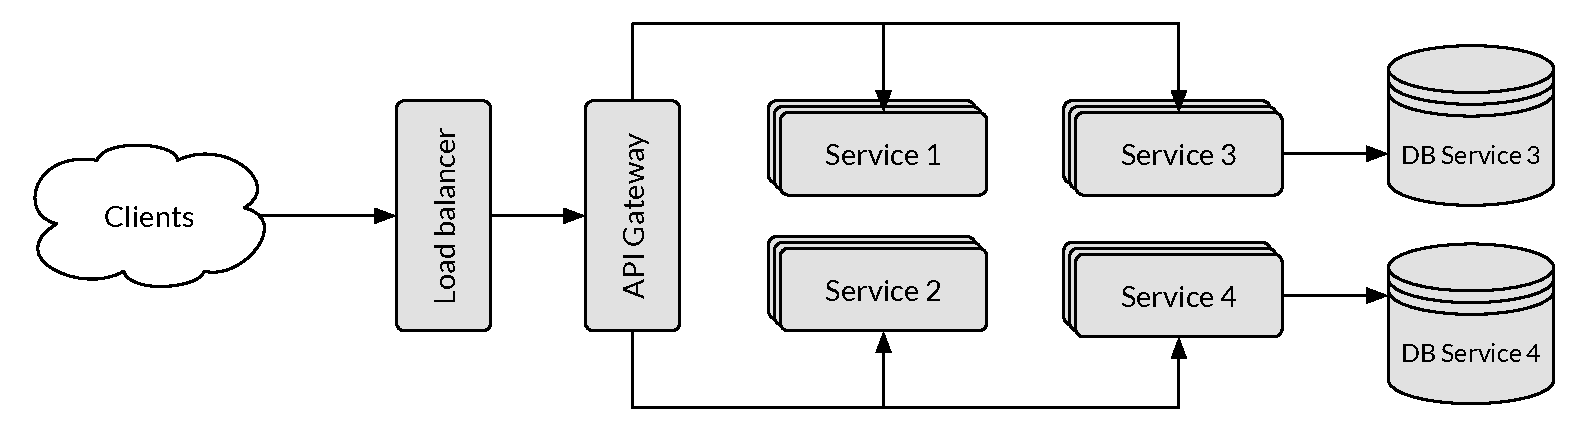
\includegraphics[width=14cm]{figures/microservices}
    \caption{Microservice Architecture}
    \label{fig:microservices}
\end{figure}

\noindent
Fowler and Lewis describe nine characteristics of a microservice architecture \cite{lewis2014microservices}. In the following section we will look into the principles and elements that characterizes a microservice architecture. A more detailed explanation of the characteristics defined by Fowler and Lewis combined with Newman's seven principles of microservices can be found in Appendix~\ref{appendix:microservices}.


\subsubsection*{Componentization via Services}
Componentization via Services refers to breaking down the architecture into services. This decomposition allows services to be independently deployable and communicate inter-process (inter-service) via 'dumb pipes' as Fowler and Lewis describe it. 

\subsubsection*{Organized around Business Capabilities}
The concept of a \textit{bounded context} from Domain Driven Design is important when organizing services. \textit{Bounded context} focus on separating entities and grouping separate context among high cohesive services, which leads to high decoupling. Microservice architecture organizes teams around functional business capabilities instead of technology layers such as UI, middleware, and database specialists. 
Conway described in 1968 that an organization's communication structure will be reflected in the way teams design their systems. 

\begin{citat} []
"[...] organizations which design  systems (in the broad sense used here) are constrained to produce designs which are copies of the communication structures of these organizations" \textbf{- Melwyn Conway, 1968} \cite[p. 31]{conway1968law} 
\end{citat}


\subsubsection*{Products not Projects}
Microservice architecture style tries to avoid the project model (software is considered done after delivery) by preferring a team owning a product over its full lifetime. Rather than looking at software as a set of functionality to be completed, there is an on-going relationship between the business and its users.


\subsubsection*{Smart Endpoints and Dumb Pipes}
Enterprise Service Bus puts a lot of \textit{smarts} into the middleware layer. The microservice community favors putting \textit{smarts} into the services instead of in the middleware. They build decoupled and highly cohesive services that own its domain logic

\subsubsection*{Decentralized Governance}
Standardizing on a single technology platform restricts the available technologies. Lewis and Fowler state: \textit{"Not every problem is a nail and not every solution is a hammer"} \cite[p. 8]{lewis2014microservices}.

\subsubsection*{Decentralized Data Management} 
One central database (Figure~\ref{fig:monolithic}) implementing the entire domain model couples services through the database. Microservice architecture embraces bounded contexts owning their own data (Figure~\ref{fig:microservices}), domain models, and only exposing necessary data through its external interfaces.


\subsubsection*{Infrastructure Automation}
The evolution of infrastructure automation techniques has reduced the operational complexity of building, deploying and operating applications. Microservices are built with the concepts of \textit{Continuous Delivery\footnote{\url{http://martinfowler.com/bliki/ContinuousDelivery.html}}} and its precursor \textit{Continuous Integration}. Two key concepts of \textit{Continuous Delivery} worth mentioning are the extensive use of automated tests and the promotion of working software pipelines to automate deployments.


\subsubsection*{Design for Failure}


A consequence of transitioning from a monolithic architecture to a microservice architecture is the shift from an intra-process integrated application to a distributed system. Any call between services can and will at some point fail, due to the non-deterministic behavior of the underlying network. Microservice architecture, therefore, needs to be designed for failure and to respond as gracefully as possible in case of error. 

\subsubsection*{Evolutionary Design}
Evolutionary design refers to the ability to cope with change. Controlling change does not necessarily mean a reduction in how frequent changes are implemented. When decomposing applications into services, the decision of how to slice up the application has to be made. Fowler and Lewis emphasize that the key property here is the notion of independent replacement and upgradability.